\documentclass[tikz,class=acmart,sigconf]{standalone}
\usepackage{xcolor}
\usepackage{xspace}

% TUM color definitions
\definecolor{TUMBlue}{cmyk}{1.00,0.43,0.00,0.00}
\definecolor{TUMRed}{cmyk}{0.10,1.00,1.00,0.10}
\definecolor{TUMGreen}{cmyk}{0.35,0.00,1.00,0.20}
\definecolor{TUMPurple}{cmyk}{0.50,1.00,0.00,0.40}
\definecolor{TUMDarkGray}{cmyk}{0.00,0.00,0.00,0.80}

% Command definitions
\newcommand{\refProfileType}[1]{\texttt{#1}}%
\newcommand{\refProfileTypeAlias}[2]{\texttt{#1}}%
\newcommand{\refProfileProperty}[2]{\texttt{#2}}%
\newcommand{\refSchemaOrg}[1]{\texttt{#1}}%
\newcommand{\refWorkflowCrate}[1]{\texttt{#1}}%
\newcommand{\rise}{RISE\xspace}%
\newcommand{\ROCrate}{RO-Crate\xspace}%
\newcommand{\wrrocLong}{Workflow Run RO-Crate\xspace}%

\pagecolor{white}

\usetikzlibrary{calc}
\usetikzlibrary{arrows.meta}
\usetikzlibrary{decorations.pathreplacing}

\usetikzlibrary{shadows}

\tikzset{
diagonal fill/.style 2 args={fill=#2, path picture={
\fill[#1, sharp corners] (path picture bounding box.south west) -|
                         (path picture bounding box.north east) -- cycle;}},
reversed diagonal fill/.style 2 args={fill=#2, path picture={
\fill[#1, sharp corners] (path picture bounding box.north west) |-
                         (path picture bounding box.south east) -- cycle;}}
}


\tikzstyle{fromSchemaOrg} = [
    draw,
    fill=TUMRed!15
]

\tikzstyle{fromProfile} = [
    draw,
    fill=TUMBlue!15
]

\tikzstyle{fromROCrate} = [
    draw,
    fill=TUMGreen!30
]

\tikzstyle{fromRunWorkflowCrate} = [
    draw,
    fill=TUMPurple!25
]

\tikzstyle{fromProfileAndSchemaOrg} = [
    diagonal fill={TUMRed!25}{TUMBlue!25}
]

\tikzstyle{fromROCrateAndSchemaOrg} = [
    diagonal fill={TUMGreen!30}{TUMRed!25}
]

\tikzstyle{fromProfileAndRunWorkflowCrate} = [
    diagonal fill={TUMPurple!25}{TUMBlue!25}
]

\tikzstyle{typeGeneral} = [
    draw=TUMDarkGray,
    fill=gray!10,
    thick,
    inner sep=0,
    font=\footnotesize
]

\tikzstyle{typeRootDataEntry} = [
    typeGeneral,
    fromROCrateAndSchemaOrg,
    minimum width=4cm,
    minimum height=1cm
]

\tikzstyle{typeExperiment} = [
    typeGeneral,
    fromProfile,
    minimum width=9cm,
    minimum height=1.5cm,
]

\tikzstyle{typeCommandFile} = [
    typeGeneral,
    fromProfile,
    minimum width=3cm,
    minimum height=1.5cm
]

\tikzstyle{typeCommandFileReset} = [
    typeGeneral,
    fill=none,
    draw=none,
    minimum width=1cm,
    minimum height=0.75cm,
    anchor=north west
]

\tikzstyle{typeCommandFileLooped} = [
    typeCommandFile,
    fromProfile
]

\tikzstyle{typeLoopRun} = [
    typeCommandFile,
    fromProfile
]

\tikzstyle{typeFile} = [
    typeGeneral,
    fromSchemaOrg,
    minimum width=1.5cm,
    minimum height=6.5cm
]

\tikzstyle{typeExperimentNode} = [
    typeGeneral,
    fromProfile,
    minimum width=2cm,
    minimum height=1cm
]

\tikzstyle{typeAuthor} = [
    typeExperimentNode,
    fromSchemaOrg
]

\tikzstyle{typeRole} = [
    typeAuthor,
    fromSchemaOrg
]

\tikzstyle{typeController} = [
    typeGeneral,
    fromSchemaOrg,
    minimum width=2.7cm,
    minimum height=1cm
]

\tikzstyle{typeOSImage} = [
    typeGeneral,
    fromProfileAndRunWorkflowCrate,
    minimum width=2cm,
    minimum height=0.75cm
]

\tikzstyle{reference} = [
    -latex,
    thick
]

\tikzstyle{listReferenceX} = [
    reference,
    double copy shadow={thick, draw=gray!50, shadow yshift=0ex},
    copy shadow={thick, draw=gray!75, shadow yshift=0ex}
]

\tikzstyle{listReferenceY} = [
    reference,
    double copy shadow={thick, draw=gray!50, shadow xshift=0ex, shadow yshift=-0.5ex},
    copy shadow={thick, draw=gray!75, shadow xshift=0ex, shadow yshift=-0.5ex}
]
\tikzstyle{listReferenceLegend} = [
    reference,
    double copy shadow={semithick, draw=gray!50, shadow xshift=0ex, shadow yshift=-0.3ex},
    copy shadow={semithick, draw=gray!75, shadow xshift=0ex, shadow yshift=-0.3ex}
]

\tikzstyle{label} = [
    font=\scriptsize\strut,
    fill=gray!30,
    inner xsep=0.05cm,
    inner ysep=0.0cm,
    outer sep=0,
    rounded corners=0.075cm
]

\tikzstyle{legend_entry_marker}=[%
    anchor=south west,
    draw,
    line width=0.35pt,
    minimum width=0.3cm,
    minimum height=0.15cm,
    inner sep=0,
    outer sep=0,
]%

\begin{document}
    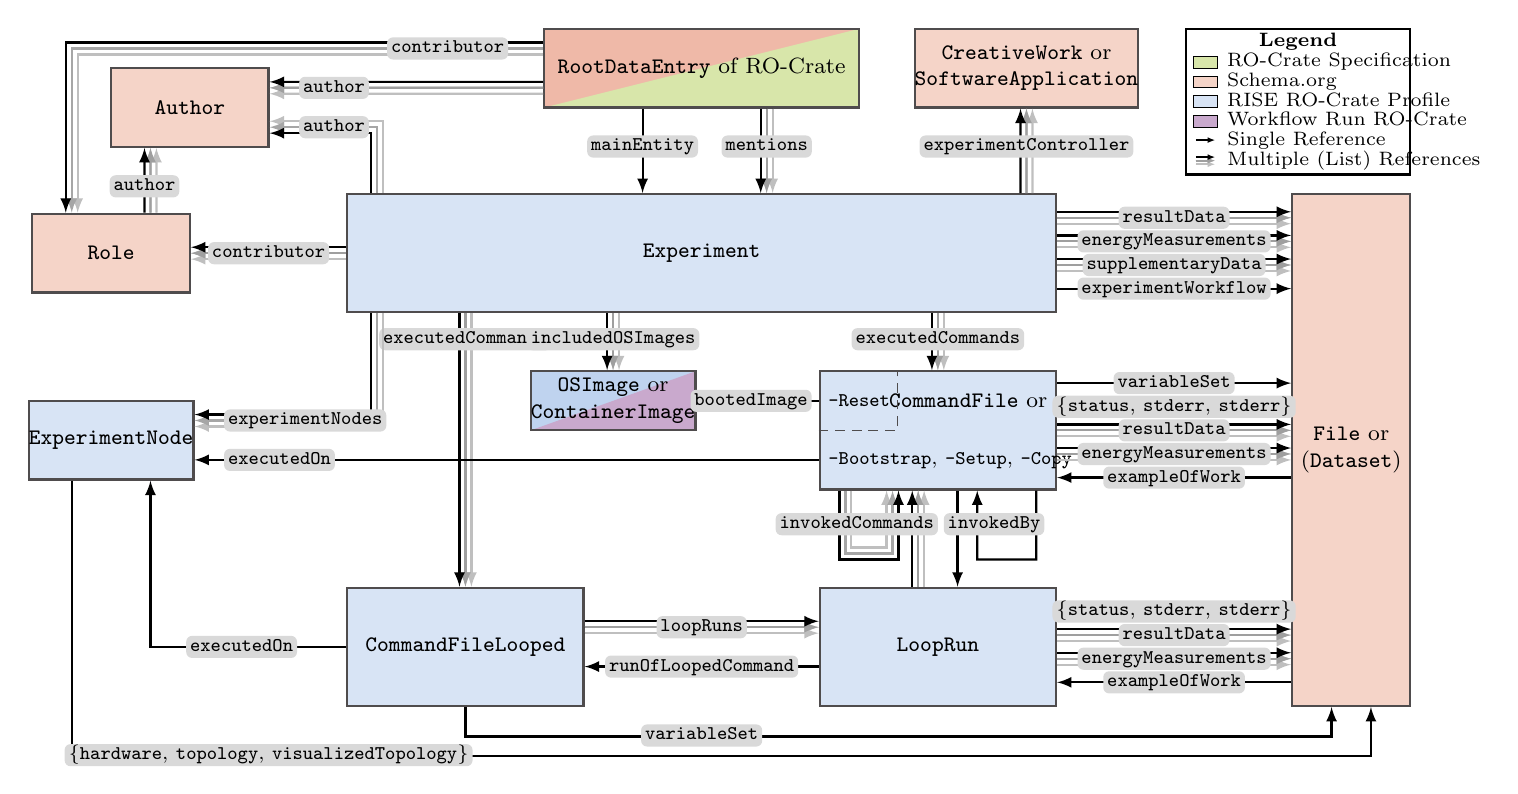
\begin{tikzpicture}

        \node[typeRootDataEntry] at (0,0.35) (RootDataEntry) {\refProfileType{RootDataEntry} of RO-Crate};
        \node[typeExperiment] at (0,-2) (Experiment) {\refProfileType{Experiment}};
        \node[typeFile,align=center] at (8.25,-4.5) (File) {\refSchemaOrg{File} or\\(\refSchemaOrg{Dataset})};

        \node[typeCommandFile,align=right] at (3,-4.25) (CommandFile) {};
        \node[font=\footnotesize, minimum width=2cm, minimum height=0.75cm, anchor=north east] at (CommandFile.north east) (typeCommandFileReset) {\refProfileType{CommandFile} or};
        \node[font=\scriptsize, minimum width=3cm, minimum height=0.75cm, anchor=south west] at (CommandFile.south west) (typeCommandFileReset) {\refProfileTypeAlias{-Bootstrap}{ComandFileBootstrap}, \refProfileTypeAlias{-Setup}{CommandFileSetup}, \refProfileTypeAlias{-Copy}{ComandFileCopy}};
        \node[typeCommandFileReset] at (CommandFile.north west) (typeCommandFileReset) {\scriptsize\refProfileTypeAlias{-Reset}{ComandFileReset}};
        \draw[draw=TUMDarkGray, dash pattern=on 3.5pt off 2.5pt] (CommandFile.west) -- ++(1,0) -- ++(0,0.75);

        \node[typeCommandFileLooped] at (-3,-7) (CommandFileLooped) {\refProfileType{CommandFileLooped}};
        \node[typeLoopRun] at (3,-7) (LoopRun) {\refProfileType{LoopRun}};
        \node[typeAuthor] at (-6.5,-0.15) (Author) {\refSchemaOrg{Author}};
        \node[typeRole] at (-7.5,-2) (Role) {\refSchemaOrg{Role}};
        \node[typeController, align=center] at (4.125,0.35) (Controller) {\refSchemaOrg{CreativeWork} or\\\refSchemaOrg{SoftwareApplication}};
        \node[typeOSImage, align=center] at (-1.125,-3.875) (OSImage) {\refProfileType{OSImage} or\\\refSchemaOrg{ContainerImage}};
        \node[typeExperimentNode] at (-7.5,-4.375) (ExperimentNode) {\refProfileType{ExperimentNode}};


        \draw[listReferenceY] ([yshift=0.25cm+0.5ex]CommandFileLooped.east) -- ([yshift=0.25cm+0.5ex]LoopRun.west)
            node[midway, label, yshift=-0.5ex]{\refProfileProperty{CommandFile}{loopRuns}};

        \draw[reference] ([yshift=-0.25cm]LoopRun.west) -- ([yshift=-0.25cm]CommandFileLooped.east)
            node[midway, label]{\refProfileProperty{CommandFile}{runOfLoopedCommand}};

        \draw[reference] (CommandFileLooped.south) -- ++(0,-0.375) -| ([xshift=-0.25cm]File.south);
        \node[label] at (0,-8.125) () {\refProfileProperty{CommandFile}{variableSet}};



        \draw[reference] ([xshift=-0.75cm]RootDataEntry.south) -- ([xshift=-0.75cm]Experiment.north)
            node[pos=1, above, yshift=0.45cm, label, label]{\refSchemaOrg{mainEntity}};
        \draw[listReferenceX] ([xshift=0.75cm]RootDataEntry.south) -- ([xshift=0.75cm]Experiment.north)
            node[pos=1, above, yshift=0.45cm, label, label, xshift=0.5ex]{\refSchemaOrg{mentions}};

        \draw[listReferenceX] ($([xshift=-0.5ex]Experiment.south -| CommandFile.north)$) -- ([xshift=-0.5ex]CommandFile.north)
            node[pos=0, below, yshift=-0.1875cm, label, xshift=0.5ex]{\refProfileProperty{CommandFile}{executedCommands}};
        \draw[listReferenceX] ($([xshift=-0.5ex]Experiment.south -| CommandFileLooped.north)$) -- ([xshift=-0.5ex]CommandFileLooped.north)
            node[pos=0, below, yshift=-0.1875cm, label, xshift=0.5ex]{\refProfileProperty{CommandFile}{executedCommands}};
        \draw[listReferenceX] ($([xshift=-0.5ex]Experiment.south -| OSImage.north)$) -- ([xshift=-0.5ex]OSImage.north)
            node[pos=0, below, yshift=-0.1875cm, label, xshift=0.5ex]{\refProfileProperty{CommandFile}{includedOSImages}};



        \draw[listReferenceX] ([xshift=4.125cm-0.5ex]Experiment.north) -- ([xshift=-0.5ex]Controller.south)
            node[pos=0, above, yshift=0.45cm, label, xshift=0.5ex] {\refProfileProperty{Experiment}{experimentController}};



        \draw[listReferenceY] ([yshift=-0.25cm+0.5ex]RootDataEntry.west) -- ([yshift=0.25cm+0.5ex]Author.east)
            node[pos=1, right, xshift=0.375cm, label, yshift=-0.5ex]{\refProfileProperty{Experiment}{author}};

        \draw[listReferenceY] ([yshift=0.5ex]Experiment.west) -- ([yshift=0.5ex]Role.east)
            node[midway, label, yshift=-0.5ex]{\refProfileProperty{Experiment}{contributor}};

        \draw[listReferenceX] ([xshift=0.5cm-0.5ex]Role.north) -- ([xshift=-0.5cm-0.5ex]Author.south)
            node[midway, label, yshift=-0.5ex]{\refProfileProperty{Experiment}{author}};



        \draw[reference, gray!50] ([yshift=0.25cm-0.5ex]RootDataEntry.west) -| ([xshift=-0.5cm+0.5ex]Role.north);
        \draw[reference, gray!70] ([yshift=0.25cm]RootDataEntry.west) -| ([xshift=-0.5cm]Role.north);
        \draw[reference] ([yshift=0.25cm+0.5ex]RootDataEntry.west) -| ([xshift=-0.5cm-0.5ex]Role.north)
            node[pos=0.1, label, yshift=-0.5ex]{\refProfileProperty{CommandFile}{contributor}};

        \draw[reference, gray!50] ([xshift=-4.125cm+0.5ex]Experiment.north) |- ([yshift=-0.25cm+0.5ex]Author.east);
        \draw[reference, gray!70] ([xshift=-4.125cm]Experiment.north) |- ([yshift=-0.25cm]Author.east);
        \draw[reference] ([xshift=-4.125cm-0.5ex]Experiment.north) |- ([yshift=-0.25cm-0.5ex]Author.east)
            node[pos=1, right, xshift=0.375cm, label, yshift=0.5ex]{\refProfileProperty{CommandFile}{author}};

        \draw[reference, gray!50] ([xshift=-4.125cm+0.5ex]Experiment.south) |- ([yshift=0.25cm-0.5ex]ExperimentNode.east);
        \draw[reference, gray!70] ([xshift=-4.125cm]Experiment.south) |- ([yshift=0.25cm]ExperimentNode.east);
        \draw[reference] ([xshift=-4.125cm-0.5ex]Experiment.south) |- ([yshift=0.25cm+0.5ex]ExperimentNode.east)
            node[pos=1, right, xshift=0.375cm, label, yshift=-0.5ex]{\refProfileProperty{CommandFile}{experimentNodes}};



        \draw[listReferenceY] ([yshift=0.45cm+0.5ex]Experiment.east) -- ($([yshift=0.45cm+0.5ex]Experiment.east -| File.west)$)
            node[midway, label, yshift=-0.5ex]{\refProfileProperty{Experiment}{resultData}};

        \draw[listReferenceY] ([yshift=0.15cm+0.5ex]Experiment.east) -- ($([yshift=0.15cm+0.5ex]Experiment.east -| File.west)$)
            node[midway, label, yshift=-0.5ex]{\refProfileProperty{Experiment}{energyMeasurements}};

        \draw[listReferenceY] ([yshift=-0.15cm+0.5ex]Experiment.east) -- ($([yshift=-0.15cm+0.5ex]Experiment.east -| File.west)$)
            node[midway, label, yshift=-0.5ex]{\refProfileProperty{Experiment}{supplementaryData}};

        \draw[reference] ([yshift=-0.45cm]Experiment.east) -- ($([yshift=-0.45cm]Experiment.east -| File.west)$)
            node[midway, label]{\refProfileProperty{Experiment}{experimentWorkflow}};



        \draw[reference] ([yshift=0.6cm]CommandFile.east) -- ($([yshift=0.6cm]CommandFile.east -| File.west)$)
            node[midway, label]{\refProfileProperty{CommandFile}{variableSet}};

        \draw[reference] ([yshift=0.3cm]CommandFile.east) -- ($([yshift=0.3cm]CommandFile.east -| File.west)$)
            node[midway, label]{\texttt{\{}\refProfileProperty{CommandFile}{status},~\refProfileProperty{CommandFile}{stderr},~\refProfileProperty{CommandFile}{stderr}\texttt{\}}};

        \draw[listReferenceY] ([yshift=0.5ex]CommandFile.east) -- ($([yshift=0.5ex]CommandFile.east -| File.west)$)
            node[midway, label, yshift=-0.5ex]{\refProfileProperty{CommandFile}{resultData}};

        \draw[listReferenceY] ([yshift=-0.3cm+0.5ex]CommandFile.east) -- ($([yshift=-0.3cm+0.5ex]CommandFile.east -| File.west)$)
            node[midway, label, yshift=-0.5ex]{\refProfileProperty{File}{energyMeasurements}};

        \draw[reference, latex-] ([yshift=-0.6cm]CommandFile.east) -- ($([yshift=-0.6cm]CommandFile.east -| File.west)$)
            node[midway, label]{\refProfileProperty{File}{exampleOfWork}};



        \draw[thick,-latex,gray!50] ([xshift=-1.25cm+1ex]CommandFile.south) -- ++([yshift=1ex]0,-0.875) -- ++([xshift=-2ex]0.75,0) -- ++([yshift=-1ex]0,0.875);
        \draw[thick,-latex,gray!70] ([xshift=-1.25cm+0.5ex]CommandFile.south) -- ++([yshift=0.5ex]0,-0.875) -- ++([xshift=-1ex]0.75,0) -- ++([yshift=-0.5ex]0,0.875);
        \draw[thick,-latex] ([xshift=-1.25cm]CommandFile.south) -- ++(0,-0.875) -- ++(0.75,0) -- ++(0,0.875);

        \draw[reference] ([xshift=1.25cm]CommandFile.south) -- ++(0,-0.875) -- ++(-0.75,0) -- ([xshift=0.5cm]CommandFile.south);

        \draw[listReferenceX] ([xshift=-0.25cm-0.5ex]LoopRun.north) -- ([xshift=-0.25cm-0.5ex]CommandFile.south)
            node[pos=0.65, label, anchor=east, xshift=0.175cm+1ex]{\refProfileProperty{CommandFile}{invokedCommands}};

        \draw[reference] ([xshift=0.25cm]CommandFile.south) -- ([xshift=0.25cm]LoopRun.north)
            node[pos=0.35, label, anchor=west, xshift=-0.175cm]{\refProfileProperty{CommandFile}{invokedBy}};



        \draw[reference] ([yshift=0.45cm]LoopRun.east) -- ($([yshift=0.45cm]LoopRun.east -| File.west)$)
            node[midway, label]{\texttt{\{}\refProfileProperty{LoopRun}{status},~\refProfileProperty{LoopRun}{stderr},~\refProfileProperty{LoopRun}{stderr}\texttt{\}}};

        \draw[listReferenceY] ([yshift=0.15cm+0.5ex]LoopRun.east) -- ($([yshift=0.15cm+0.5ex]LoopRun.east -| File.west)$)
            node[midway, label, yshift=-0.5ex]{\refProfileProperty{CommandFile}{resultData}};

        \draw[listReferenceY] ([yshift=-0.15cm+0.5ex]LoopRun.east) -- ($([yshift=-0.15cm+0.5ex]LoopRun.east -| File.west)$)
            node[midway, label, yshift=-0.5ex]{\refProfileProperty{File}{energyMeasurements}};

        \draw[reference, latex-] ([yshift=-0.45cm]LoopRun.east) -- ($([yshift=-0.45cm]LoopRun.east -| File.west)$)
            node[midway, label]{\refProfileProperty{File}{exampleOfWork}};



        \draw[reference] ([yshift=0.375cm]CommandFile.west) -- (OSImage.east)
            node[pos=0, xshift=-0.09cm, left, label]{\refProfileProperty{CommandFile}{bootedImage}};



        \draw[reference] ([yshift=-0.375cm]CommandFile.west) -- ([yshift=-0.25cm]ExperimentNode.east)
            node[pos=1, right, xshift=0.375cm, label]{\refProfileProperty{CommandFile}{executedOn}};

        \draw[reference] (CommandFileLooped.west) -| ([xshift=0.5cm]ExperimentNode.south)
            node[pos=0, xshift=-0.625cm, left, label]{\refProfileProperty{CommandFile}{executedOn}};

        \draw[reference] ([xshift=-0.5cm]ExperimentNode.south) -- ++(0,-3.5) -| ([xshift=0.25cm]File.south);
        \node[label] at (-5.5,-8.375) () {\texttt{\{}\refProfileProperty{ExperimentNode}{hardware},~\refProfileProperty{ExperimentNode}{topology},~\refProfileProperty{ExperimentNode}{visualizedTopology}\texttt{\}}};



        \node[draw, anchor=north east, minimum width=2.85cm, minimum height=1.85cm, thick, inner sep=0,outer sep=0] at (9,0.85) (legend) {};
        \node[anchor=north, font=\scriptsize\bfseries, inner sep=0.05cm] at (legend.north) () {Legend};

        \node[legend_entry_marker, fromROCrate] at ([xshift=0.1cm, yshift=1.35cm]legend.south west) (legend_files) {};
        \node[font=\scriptsize, anchor=west] at (legend_files.east) () {RO-Crate Specification\strut};

        \node[legend_entry_marker, fromSchemaOrg] at ([xshift=0.1cm, yshift=1.1cm]legend.south west) (legend_files) {};
        \node[font=\scriptsize, anchor=west] at (legend_files.east) () {Schema.org\strut};

        \node[legend_entry_marker, fromProfile] at ([xshift=0.1cm, yshift=0.85cm]legend.south west) (legend_files) {};
        \node[font=\scriptsize, anchor=west] at (legend_files.east) () {\rise~\ROCrate~Profile\strut};

        \node[legend_entry_marker, fromRunWorkflowCrate] at ([xshift=0.1cm, yshift=0.6cm]legend.south west) (legend_files) {};
        \node[font=\scriptsize, anchor=west] at (legend_files.east) () {\wrrocLong\strut};

        \draw[reference, -{Latex[scale=0.5]}, semithick] ([xshift=0.125cm, yshift=0.425cm+0.075ex]legend.south west) -- ++(0.25,0)
            node[font=\scriptsize, anchor=west, xshift=0.025cm, yshift=-0.075ex] {Single Reference\strut};

        \draw[listReferenceLegend, -{Latex[scale=0.5]}, semithick] ([xshift=0.125cm, yshift=0.175cm+0.3ex]legend.south west) -- ++(0.25,0)
            node[font=\scriptsize, anchor=west, xshift=0.025cm,yshift=-0.3ex] {Multiple (List) References\strut};

    \end{tikzpicture}
\end{document}
